\documentclass{beamer}\usepackage[]{graphicx}\usepackage[]{color}
% maxwidth is the original width if it is less than linewidth
% otherwise use linewidth (to make sure the graphics do not exceed the margin)
\makeatletter
\def\maxwidth{ %
  \ifdim\Gin@nat@width>\linewidth
    \linewidth
  \else
    \Gin@nat@width
  \fi
}
\makeatother

\definecolor{fgcolor}{rgb}{0.345, 0.345, 0.345}
\newcommand{\hlnum}[1]{\textcolor[rgb]{0.686,0.059,0.569}{#1}}%
\newcommand{\hlstr}[1]{\textcolor[rgb]{0.192,0.494,0.8}{#1}}%
\newcommand{\hlcom}[1]{\textcolor[rgb]{0.678,0.584,0.686}{\textit{#1}}}%
\newcommand{\hlopt}[1]{\textcolor[rgb]{0,0,0}{#1}}%
\newcommand{\hlstd}[1]{\textcolor[rgb]{0.345,0.345,0.345}{#1}}%
\newcommand{\hlkwa}[1]{\textcolor[rgb]{0.161,0.373,0.58}{\textbf{#1}}}%
\newcommand{\hlkwb}[1]{\textcolor[rgb]{0.69,0.353,0.396}{#1}}%
\newcommand{\hlkwc}[1]{\textcolor[rgb]{0.333,0.667,0.333}{#1}}%
\newcommand{\hlkwd}[1]{\textcolor[rgb]{0.737,0.353,0.396}{\textbf{#1}}}%
\let\hlipl\hlkwb

\usepackage{framed}
\makeatletter
\newenvironment{kframe}{%
 \def\at@end@of@kframe{}%
 \ifinner\ifhmode%
  \def\at@end@of@kframe{\end{minipage}}%
  \begin{minipage}{\columnwidth}%
 \fi\fi%
 \def\FrameCommand##1{\hskip\@totalleftmargin \hskip-\fboxsep
 \colorbox{shadecolor}{##1}\hskip-\fboxsep
     % There is no \\@totalrightmargin, so:
     \hskip-\linewidth \hskip-\@totalleftmargin \hskip\columnwidth}%
 \MakeFramed {\advance\hsize-\width
   \@totalleftmargin\z@ \linewidth\hsize
   \@setminipage}}%
 {\par\unskip\endMakeFramed%
 \at@end@of@kframe}
\makeatother

\definecolor{shadecolor}{rgb}{.97, .97, .97}
\definecolor{messagecolor}{rgb}{0, 0, 0}
\definecolor{warningcolor}{rgb}{1, 0, 1}
\definecolor{errorcolor}{rgb}{1, 0, 0}
\newenvironment{knitrout}{}{} % an empty environment to be redefined in TeX

\usepackage{alltt}
\usepackage{../371g-slides}
\title{Introduction to predictive analytics}
\subtitle{Lecture 1}
\author{STA 371G}
% \setbeameroption{show notes on second screen}
\IfFileExists{upquote.sty}{\usepackage{upquote}}{}
\begin{document}



  \frame{\maketitle}

  % Show outline at beginning of each section
  \AtBeginSection[]{
    \begin{frame}<beamer>
      \tableofcontents[currentsection]
    \end{frame}
  }

  %%%%%%% Slides start here %%%%%%%

  \begin{darkframes}
    \begin{frame}{Course goals}
      \begin{itemize}
        \item Use regression and time series analysis to build predictive models
        \item Create decision tree models to systematize business decision-making
        \item Utilize simulations to forecast outputs based on uncertain inputs
        \item Given a new business situation, select an appropriate analysis, carry it out, and effectively communicate the results
        \item \alert{This is a practical course!}
      \end{itemize}
    \end{frame}

    \begin{frame}{About the course staff}
      \begin{itemize}
        \item Instructor: \textbf{Brian Lukoff, Ph.D.} (he/him/his)
          \begin{itemize}
            \item Office hours: MW 9:30-10:30 AM
            \item Course questions: \texttt{sta371g-lukoff@austin.utexas.edu}
            \item Personal contact: \texttt{brian.lukoff@utexas.edu} or 415-652-8853
          \end{itemize}
        \item TAs and office hours:
      \end{itemize}

      \vspace{0.2in}
      \hspace*{-0.3in}\begin{tabular}{cccc}
        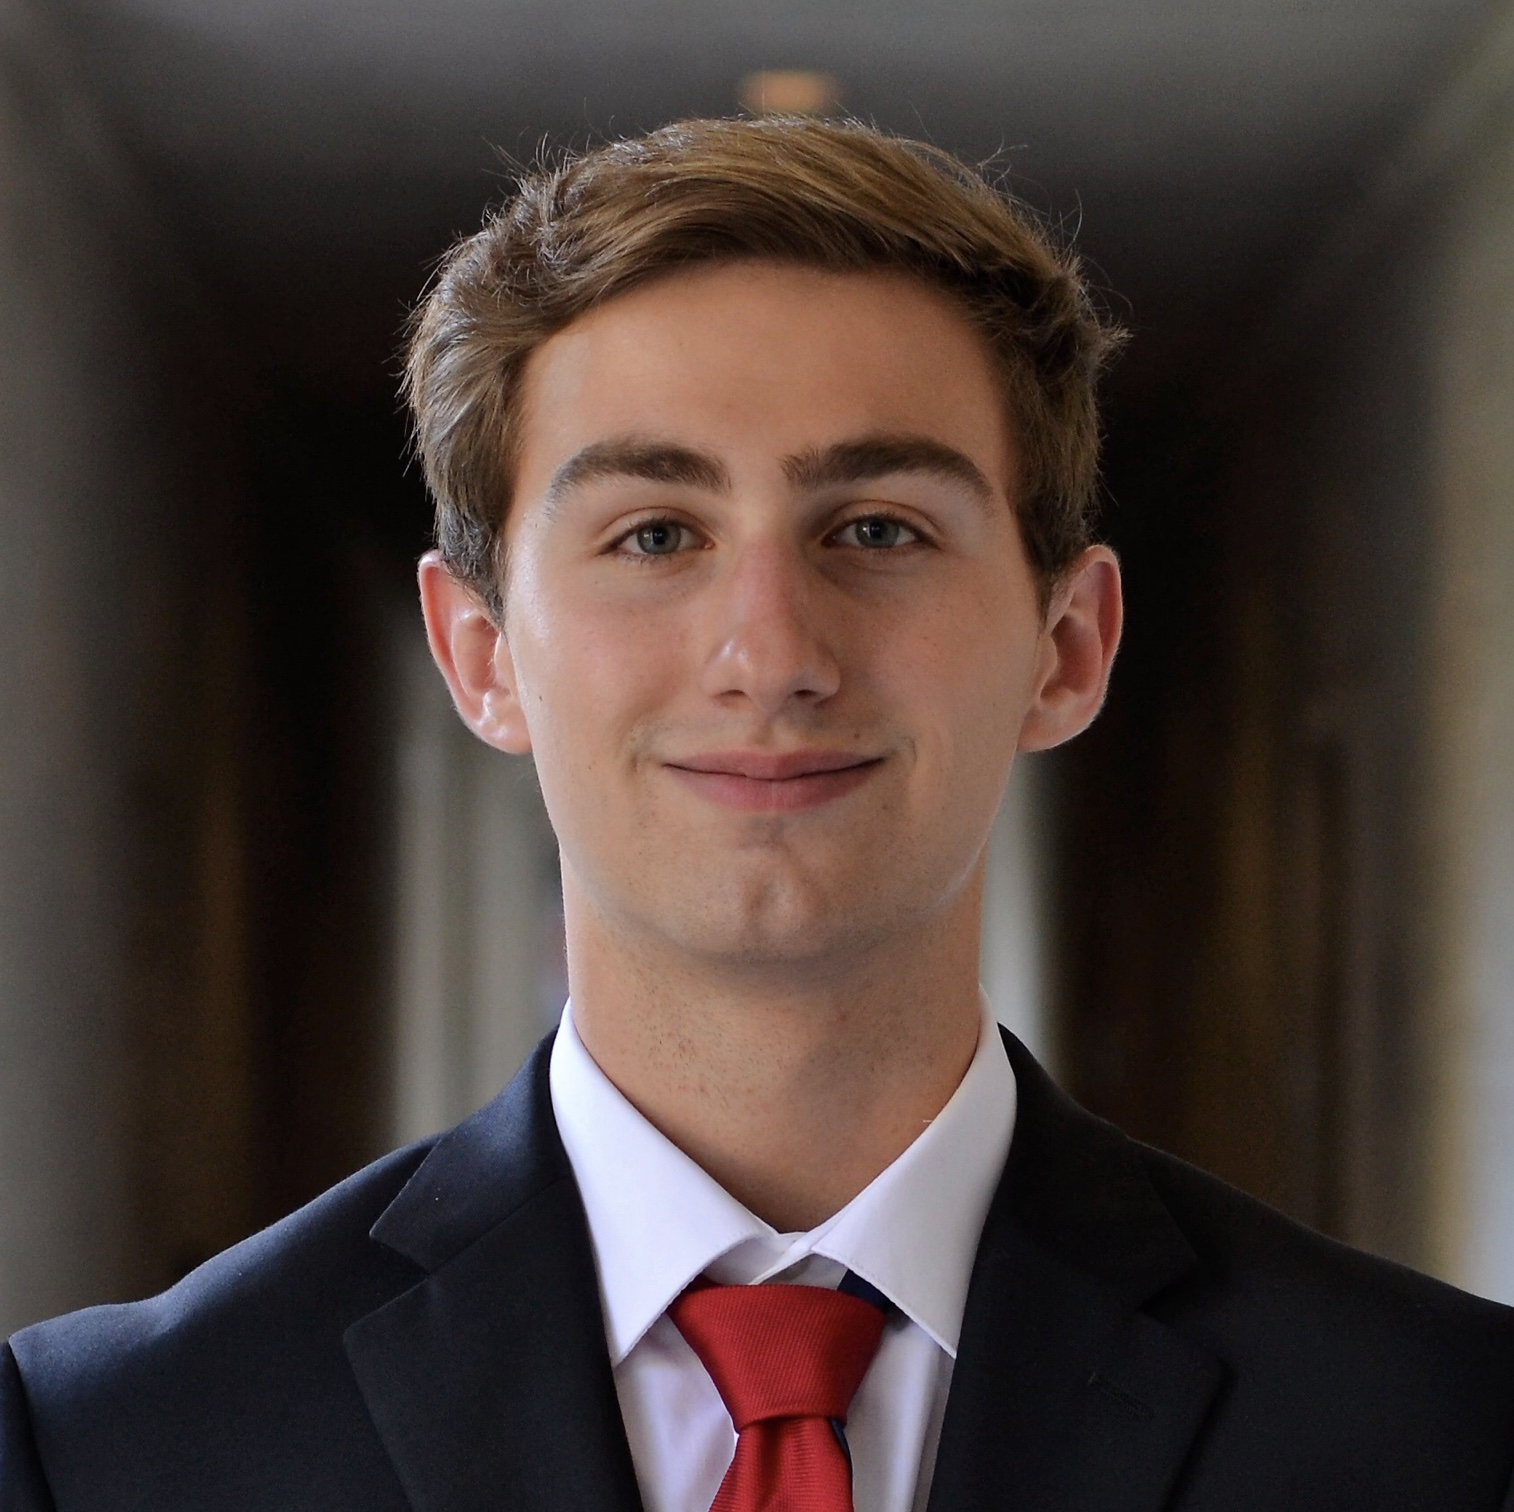
\includegraphics[width=0.7in]{holden} &
        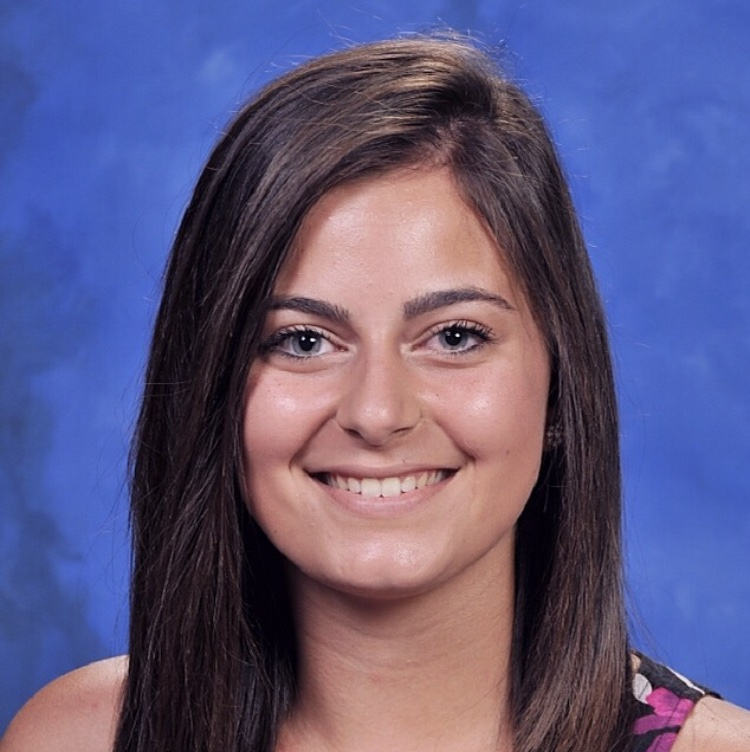
\includegraphics[width=0.7in]{michelle} &
        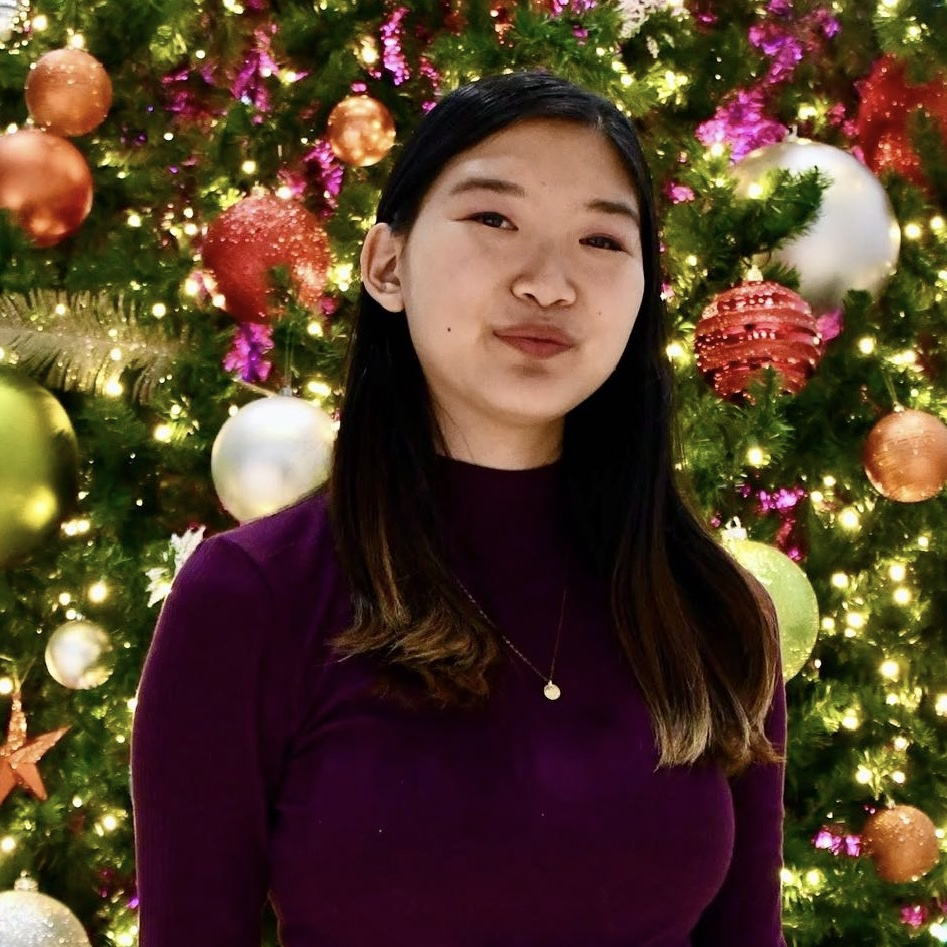
\includegraphics[width=0.7in]{meryl} &
        
\includegraphics[width=0.7in]{leyang} \\
        Holden Archer & Michelle Chahda  & Meryl Xiong & Leyang Xu \\
        M 3:30-6:30 PM & Th 3:30-6:30 PM & MW 11-12:30 PM & F 2:00-5:00 PM  \\
      \end{tabular}
    \end{frame}

    \begin{frame}{Who am I?}
      \begin{itemize}
        \item \textbf{Educator:} Teaching statistics at McCombs since 2014; previously taught at Harvard University and Boston University
        \item \textbf{Entrepreneur:} Currently co-founder and CEO of Perusall; formerly co-founder and CEO of Learning Catalytics (acquired by Pearson)
        \item \textbf{Engineer/statistician:} Software engineering/analytics background
      \end{itemize}
    \end{frame}

    \section{Find someone who...}

    \begin{frame}{}
      \begin{center}
        Your group gets points if someone in your breakout room matches the characteristic below. 
        The goal is for your group to get the most points.
        Each member of your group can only be used \alert{once}!
        \vfill
        The winning group will be crowned the STA 371G Find Someone Who Champion$^{\text{TM}}$ (SFSWC$^{\text{TM}}$).
      \end{center}
    \end{frame}

    \begin{frame}
      \begin{multicols}{2}
        \begin{itemize}
          \item [1 pt] Has been to a UT football game
          \item [1 pt] Has been to Torchy's Tacos
          \item [1 pt] Plays a musical instrument
          \item [1 pt] Doesn't like asparagus
          \item [1 pt] Has ridden a bike
          \item [1 pt] Has worn earrings
          \item [1 pt] Is an only child
          \item [2 pts] Has been to a honky tonk
          \item [2 pts] Has met a celebrity
          \item [2 pts] Was born outside of Texas
          \item [2 pts] Was born outside of the US
          \item [2 pts] Has a tattoo
          \item [2 pts] Can do a Rubik's cube        
          \item [3 pts] Watches \emph{Jersey Shore: Family Vacation}
          \item [3 pts] Can wiggle their ears
          \item [3 pts] Thinks statistics is awesome (really!)
          \item [3 pts] Voted in a national election (US or non-US) in 2020
        \end{itemize}
      \end{multicols}
    \end{frame}

    \section{Course logistics}

    \begin{frame}{Canvas}
      \begin{itemize}
        \item Access at \url{canvas.utexas.edu}
        \item This is your home base for the course
        \item Make sure you can log in and are enrolled in STA 371G in Canvas
      \end{itemize}
    \end{frame}


    \begin{frame}{Textbook}
      \begin{columns}[onlytextwidth]
        \column{.6\textwidth}
        \begin{itemize}
          \item Access the textbook as an eBook through MyStatLab OR buy a hardcover or looseleaf textbook (Sharpe, \emph{Business Statistics}, 4th ed) that includes a MyStatLab access code
        \end{itemize}
        \column{.35\textwidth}
          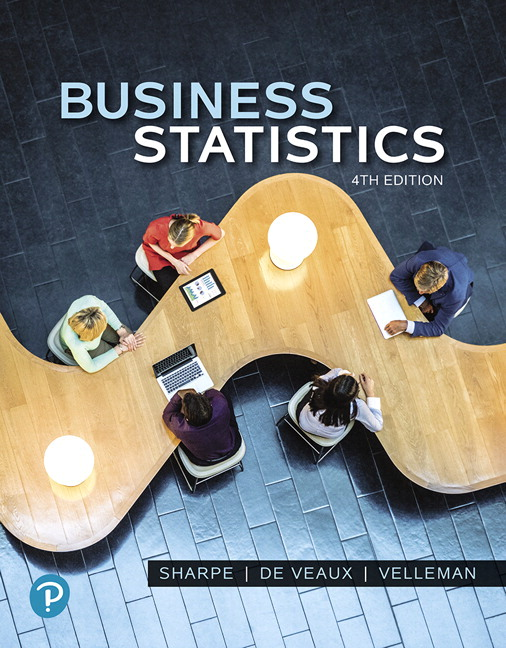
\includegraphics[width=1.5in]{textbook}
      \end{columns}
    \end{frame}


    \begin{frame}{Using Zoom}
      \begin{itemize}
        \item Make sure to join using your UT Zoom account (you should \emph{not} find yourself in the waiting room)
        \item Stay muted during class, unless you are called on
        \item Raise your hand (in the Participant window) to ask questions
        \item Feel free to use the chat (Leyang will monitor during class)
      \end{itemize}
    \end{frame}


    \begin{frame}{Class structure}
      \begin{itemize}
        \item Understanding the concepts really only comes from practice
        \item Class will be synchronous; class time will be divided between lecture and practice
        \item We will use \alert{Learning Catalytics} so you can practice the concepts during class
        \item No cost to use this
        \item Graded on participation, not correctness; answer 75\% of the questions to get 100\% of the credit
      \end{itemize}
    \end{frame}

    
    \begin{frame}{Let's try out Learning Catalytics}
      \begin{enumerate}
        \item Go to Canvas, and click \alert{MyLab and Mastering} in the left sidebar. Log in with your Pearson account, or create one.
        \item In the Learning Catalytics box, click \alert{Join Session in Progress}.
        \item Answer the question there!
      \end{enumerate}
    \end{frame}


    \begin{frame}{Homework}
      \begin{columns}[onlytextwidth]
        \column{.5\textwidth}
          \begin{itemize}
            \item Why homework?
            \item 12 homework assignments during the semester, due Mondays
            \item We will use \alert{MyStatLab} for online homework; purchase and register through Canvas (you'll get a 2-week free trial)
          \end{itemize}
        \column{.4\textwidth}
          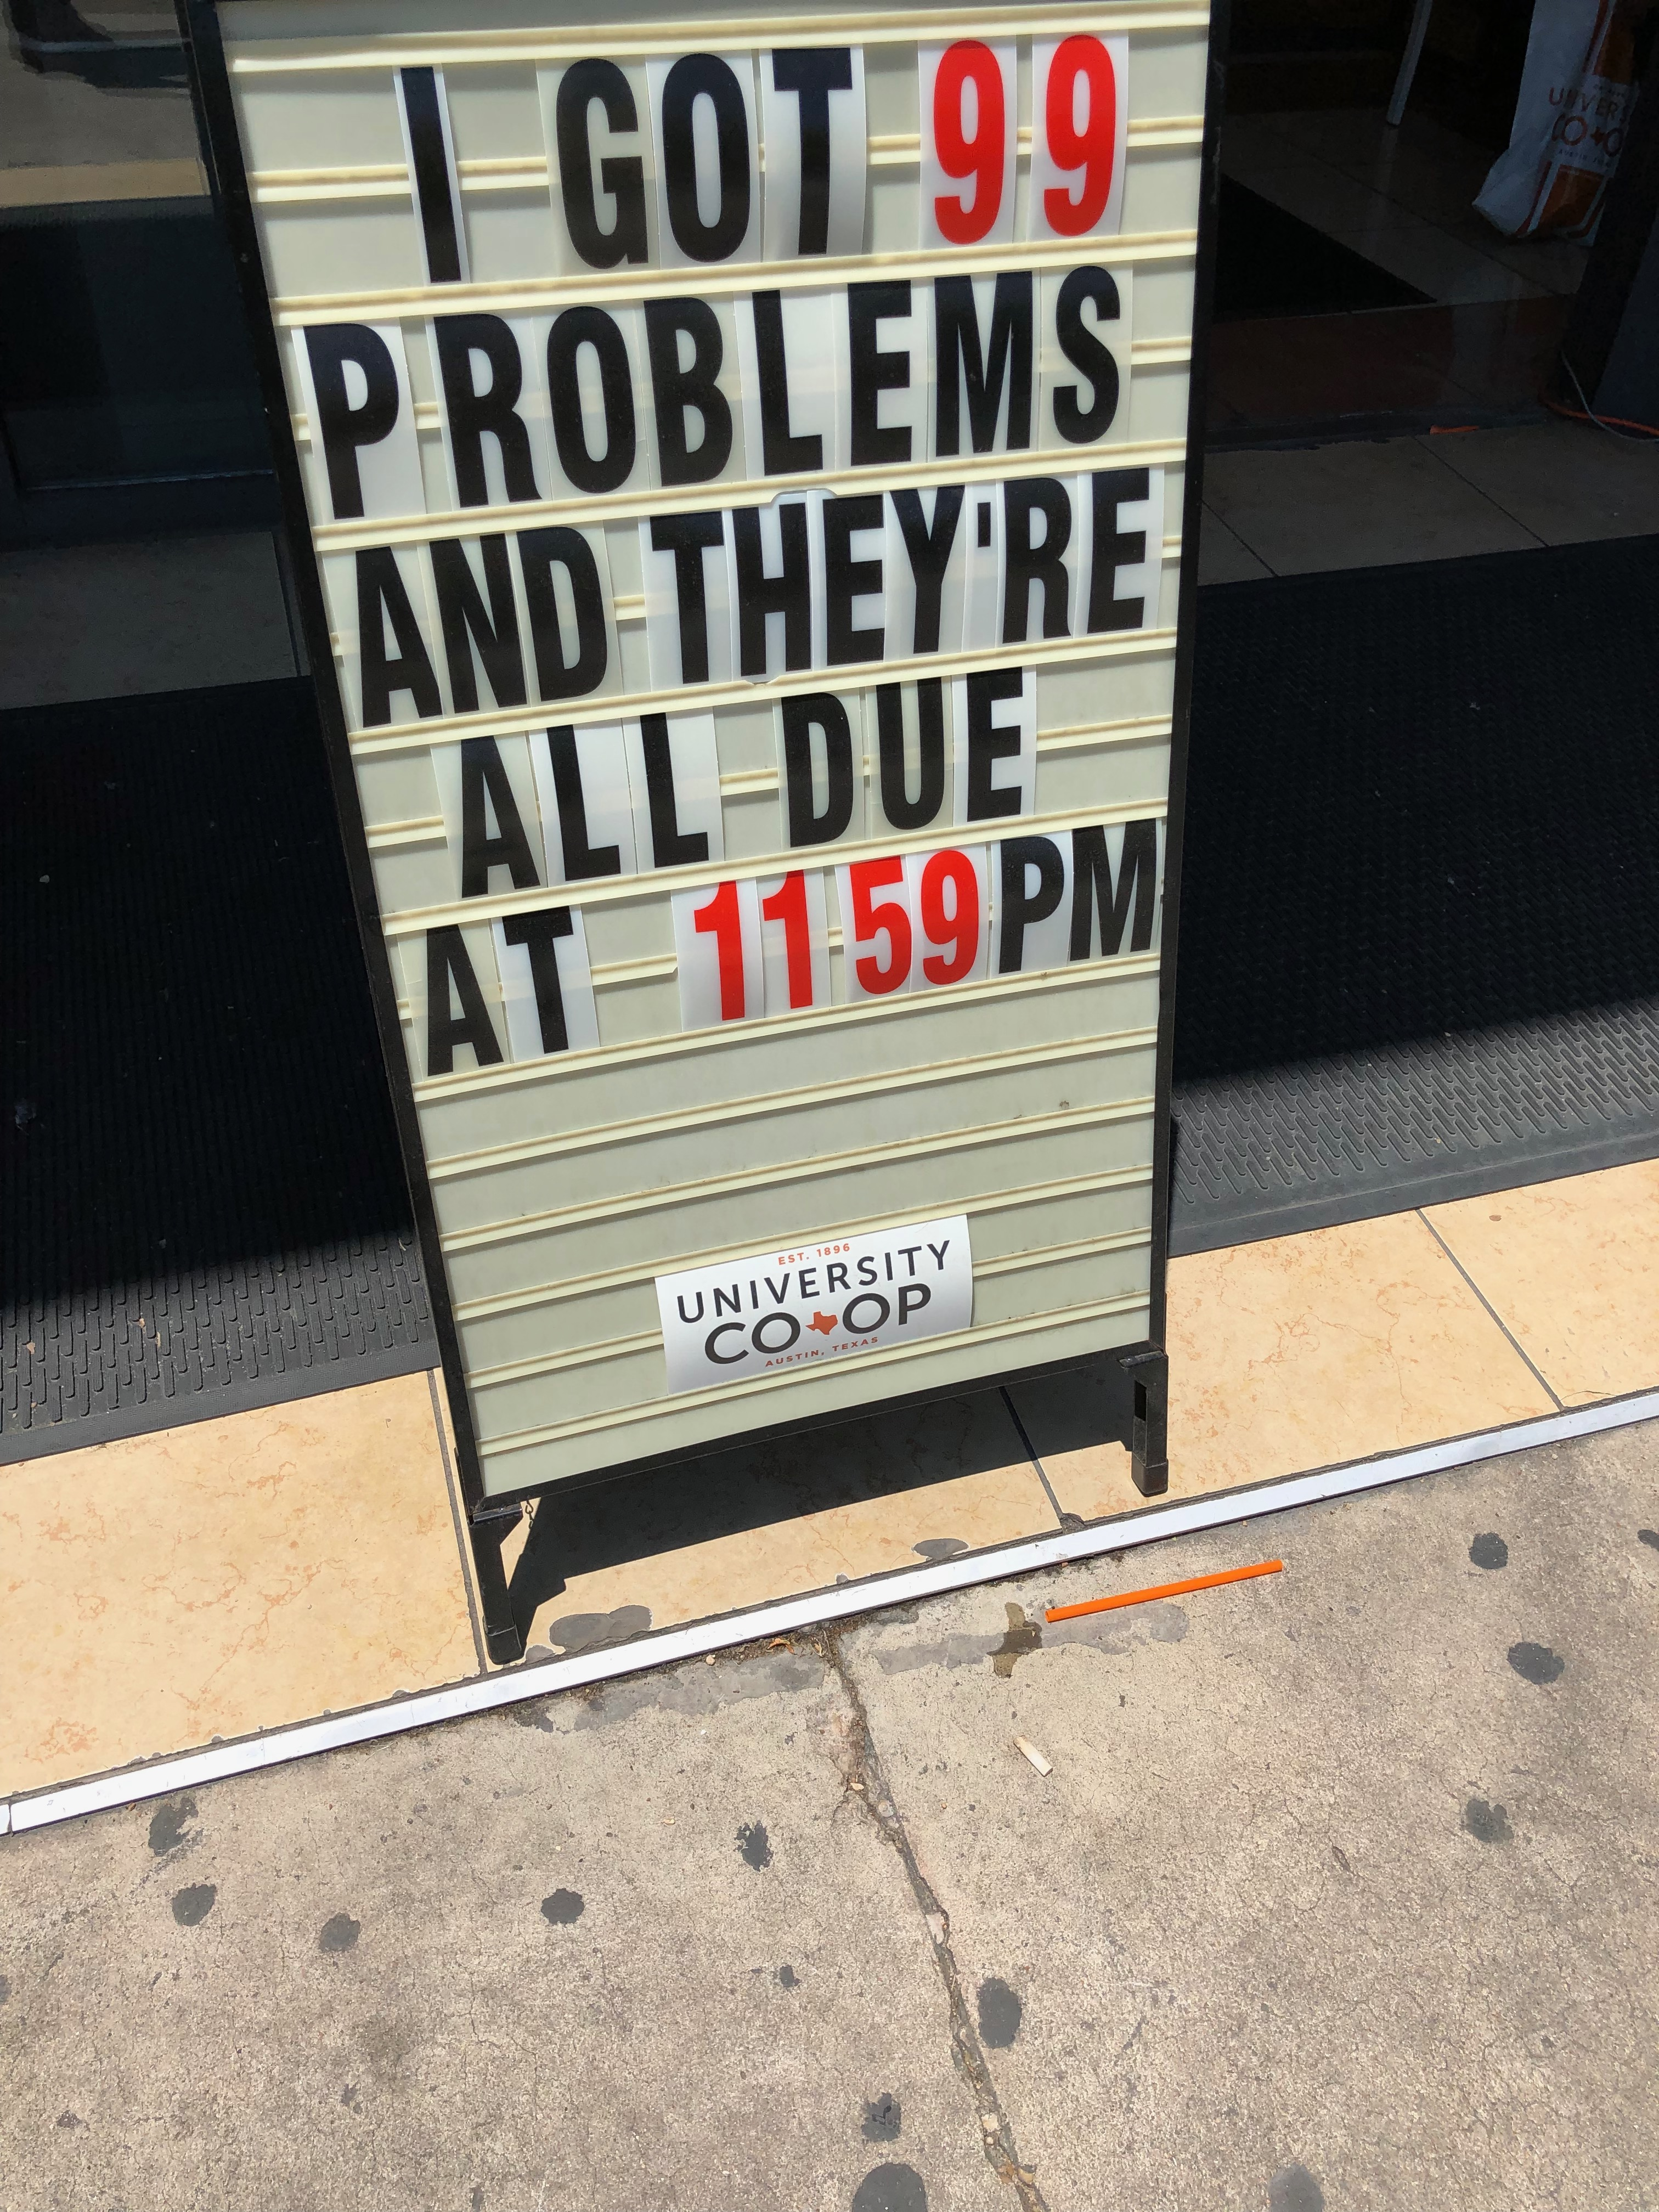
\includegraphics[width=1.5in]{99problems}
      \end{columns}
    \end{frame}
    

    \begin{frame}{Statistical computing}
      \begin{columns}[onlytextwidth]
        \column{.6\textwidth}
          \begin{itemize}
            \item We will use \alert{R} for statistical analysis throughout the course
            \item This is industrial-strength, state-of-the-art, and free software for statistical computing
            \item We will access R through \alert{RStudio}, a graphical interface for R
            \item Download R and RStudio at \url{rstudio.com}
          \end{itemize}
        \column{.3\textwidth}
          
\includegraphics[width=1in]{R}
      \end{columns}
    \end{frame}

    \begin{frame}{Quizzes}
      \begin{itemize}
        \item Short weekly quizzes on Tuesdays at 6:30 PM
        \item No midterm or final exams!
        \item Quizzes are cumulative and may include questions from earlier in the semester
        \item Take quizzes on your own (quizzes are automatically analyzed for patterns of suspicious behavior)
        \item You'll have access to R during every quiz
        \item I will drop the lowest of your quiz scores
      \end{itemize}
    \end{frame}

    \begin{frame}{Team project}
      \begin{itemize}
        \item You will apply regression techniques (we'll learn about this!) to build a predictive model for an interesting data set
        \item Six deliverables throughout the semester:
        \begin{enumerate}
          \item Initial proposal (March 4)
          \item Literature review (March 11)
          \item Final proposal (April 1)
          \item Exploratory data analysis (April 15)
          \item PowerPoint deck (April 29)
          \item Presentation to class (May 3-5 \& 18)
        \end{enumerate}
      \end{itemize}
    \end{frame}

    \begin{frame}{Academic integrity}
      \begin{itemize}
        \item Academic integrity (scholastic honesty) is an important prerequisite for academic achievement (a degree obtained by cheating doesn't mean anything, and cheating devalues the whole process for everyone!)
        \item Do not collaborate on projects (outside of your team project group) or on quizzes
        \item Don't be afraid to ask if you have a question about what is allowed
      \end{itemize}
    \end{frame}

    \begin{frame}{Grading}
      \begin{center}
        \begin{tabular}{ll}
          Quizzes             & \textbf{50\%} \\
          Project             & \textbf{25\%} \\
          Homework            & \textbf{15\%} \\
          Learning Catalytics & \textbf{10\%}  \\
        \end{tabular}
      \end{center}
    \end{frame}

    \begin{frame}{PLUS (Peer-Led Undergraduate Studying)}
      \begin{columns}[onlytextwidth]
        \column{.4\textwidth}
          \begin{itemize}
            \item Weekly, student-run study groups
            \item You can apply to be a facilitator or just participate in any of the sessions
            \item Students who attend more PLUS sessions tend to get higher grades!
            \item PLUS will begin in the third week of the semester
          \end{itemize}
        \column{.5\textwidth}
          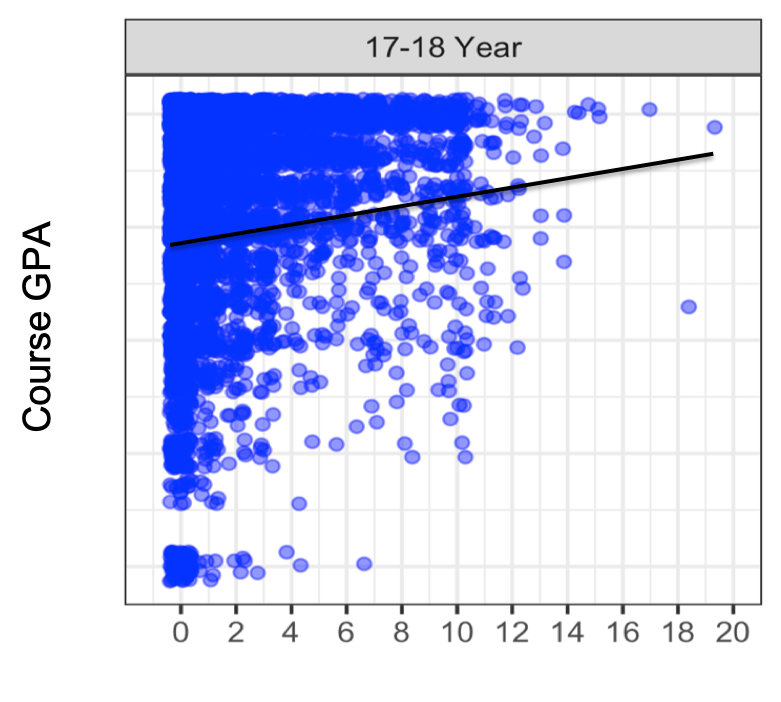
\includegraphics[width=2in]{plus}
      \end{columns}
    \end{frame}

    \begin{frame}{How to get an A in STA 371G}
      \begin{itemize}
        \item Work on more problems than are assigned in the homework; can find problems in the book and on MyStatLab
        \item Consider attending the PLUS sessions
        \item Get help when you need it
          \begin{itemize}
            \item My office hours (after every class, until 10:30 AM)
            \item TA office hours (see syllabus for schedule)
            \item Post questions on Piazza (accessible through Canvas)
            \item E-mail the staff address (\texttt{sta371g-lukoff@austin.utexas.edu}) to ask questions
            \item E-mail me directly (\texttt{brian.lukoff@utexas.edu}) for private questions or to set up an appointment
          \end{itemize}
      \end{itemize}
    \end{frame}

    \section{Let's do some statistics, yo}

    \begin{frame}{Purpose of a model}
      \begin{itemize}
        \item \textbf{Make a prediction} about one variable based on the others
        \item \textbf{Understand the relationships} between the variables
      \end{itemize}
    \end{frame}

    \begin{frame}{Data analysis process}
      \begin{center}
        \tikzstyle{block} = [rectangle, draw, fill=darkgray,
            rounded corners, minimum height=2em]
        \tikzstyle{line} = [draw, -latex']

        \begin{tikzpicture}[node distance = 1.4cm, auto]
          \node [block] (define) {define problem};
          \node [block, below of=define] (explore) {explore the data};
          \node [block, below of=explore] (build) {build model};
          \node [block, below of=build] (evaluate) {evaluate model};
          \node [block, below of=evaluate] (conclude) {make conclusions};
          \path [line] (define) -- (explore);
          \path [line] (explore) -- (build);
          \path [line] (build) -- (evaluate);
          \path [line] (evaluate) -- (conclude);
        \end{tikzpicture}
      \end{center}
    \end{frame}

    \begin{frame}{Define the problem}
      \begin{center}
        What personal characteristics about an instructor do you think are predictive of the scores they receive on student evaluations?
      \end{center}
    \end{frame}

    \begin{frame}
      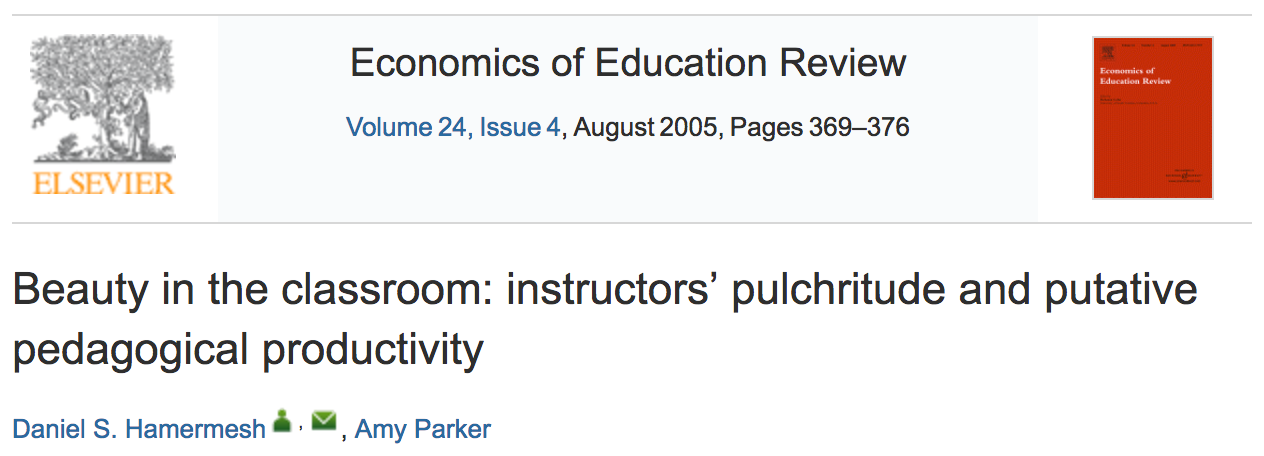
\includegraphics[width=\textwidth]{hamermesh}
    \end{frame}

    \begin{frame}{Hamermesh \& Parker (2005) data set}
      \begin{itemize}
        \item Student evaluations of $N=463$ instructors at UT Austin, 2000-2002
        \item For each instructor:
          \begin{itemize}
            \item \textbf{beauty}: average score from a six-student panel)
            \item \textbf{gender}: male or female
            \item \textbf{credits}: single- or multi-credit course
            \item \textbf{age}: age of instructor
            \item (and more...)
          \end{itemize}
      \end{itemize}
    \end{frame}

    

    \begin{frame}{Explore the data}
\begin{knitrout}
\definecolor{shadecolor}{rgb}{0.969, 0.969, 0.969}\color{fgcolor}
\includegraphics[width=\maxwidth]{/tmp/figures/unnamed-chunk-3-1} 

\end{knitrout}
    \end{frame}

    \begin{frame}{Explore the data}
\begin{knitrout}
\definecolor{shadecolor}{rgb}{0.969, 0.969, 0.969}\color{fgcolor}
\includegraphics[width=\maxwidth]{/tmp/figures/unnamed-chunk-4-1} 

\end{knitrout}
    \end{frame}

    \begin{frame}{Explore the data}
\begin{knitrout}
\definecolor{shadecolor}{rgb}{0.969, 0.969, 0.969}\color{fgcolor}
\includegraphics[width=\maxwidth]{/tmp/figures/unnamed-chunk-5-1} 

\end{knitrout}
    \end{frame}

    \begin{frame}{Explore the data}
\begin{knitrout}
\definecolor{shadecolor}{rgb}{0.969, 0.969, 0.969}\color{fgcolor}
\includegraphics[width=\maxwidth]{/tmp/figures/unnamed-chunk-6-1} 

\end{knitrout}
    \end{frame}

    \begin{frame}{Build the model}
      
      \begin{center}
        A regression model lets us create a model that incorporates all of these relationships to best predict evaluation scores:
        \[
          \widehat{\text{eval}} =
            4.13 +
            0.16 \cdot \text{beauty} -
            0.2 \cdot \text{female} +
            0.58 \cdot \text{credits} +
            0 \cdot \text{age}
        \]

        \pause

        We predict a 40-year-old female, with a beauty score of 2, teaching a multi-credit course would get an evaluation score of
        \[
          \widehat{\text{eval}} = 4.13 + 0.16 \cdot 2 - 0.2 \cdot 1 + 0.58 \cdot 0 = 4.18.
        \]

      \end{center}
    \end{frame}

    \begin{frame}{Evaluate the model}
      How could you evaluate the quality of this model?
    \end{frame}

    \begin{frame}{Can we do better?}
      Do you see a difference between men (blue) and women (red)?

\begin{knitrout}
\definecolor{shadecolor}{rgb}{0.969, 0.969, 0.969}\color{fgcolor}
\includegraphics[width=\maxwidth]{/tmp/figures/unnamed-chunk-8-1} 

\end{knitrout}
    \end{frame}

    \begin{frame}{Can we do better?}
      Do you see a difference between men (blue) and women (red)?

\begin{knitrout}
\definecolor{shadecolor}{rgb}{0.969, 0.969, 0.969}\color{fgcolor}
\includegraphics[width=\maxwidth]{/tmp/figures/unnamed-chunk-9-1} 

\end{knitrout}
    \end{frame}

    \begin{frame}{Five for the weekend}
      \begin{enumerate}
        \item Read the syllabus
        \item Do the first reading assignment (\S 5.1-5.8, on probability)
        \item Install R and RStudio on your computer (instructions on Canvas)
        \item Get registered with MyStatLab (access through Canvas)
        \item Watch the video message from Michelle about PLUS, and apply to be a facilitator if you are interested
      \end{enumerate}
    \end{frame}

  \end{darkframes}
\end{document}
